%\documentclass{vldb}
\documentclass{sig-alternate}
%\documentclass[12pt,letterpaper]{article}
%\documentclass[12pt]{extreport}
%\documentstyle[amsmath,amsthm,amssymb,twocolumn]{article}
%\newcommand{\mytitle}{Evaluating the Crowd with Confidence}

%\usepackage{amsmath}
\makeatletter
\let\@copyrightspace\relax
\makeatother
\pdfpagewidth=8.5in
\pdfpageheight=11in

\renewcommand{\baselinestretch}{1.0}

\usepackage{enumitem}
\usepackage{times}
\usepackage{subfigure}
\usepackage{amsmath,amssymb}
\usepackage{graphicx,color}
\usepackage{verbatim}
\usepackage{framed}
\usepackage[ruled,vlined]{algorithm2e}
\usepackage{framed}

\newtheorem{theorem}{Theorem}
\newtheorem{lemma}{Lemma}
\newtheorem{definition}{Definition}
\newtheorem{example}[definition]{Example}
\newcounter{prob}
\newtheorem{problem}[prob]{Problem}

\newcommand{\agp}[1]{ \textcolor{red}{\bf ||Ins: #1||}}
\newcommand{\agpdel}[1]{\textcolor{blue}{\bf ||Del: #1||}}

\newcommand{\squishlist}{
   \begin{list}{$\bullet$}
    { \setlength{\itemsep}{0pt}
      \setlength{\parsep}{2pt}
      \setlength{\topsep}{2pt}
      \setlength{\partopsep}{0pt}
    }
}
\newcommand{\stitle}[1]{\vspace{0.5em}\noindent\textbf{#1}}
\newcommand{\squishend}{\end{list}}
\newcommand{\eat}[1]{}
\newcommand{\papertext}[1]{#1}
\newcommand{\techreporttext}[1]{}

\title{Interactive Summarization of Relational Tables}

\author{
Manas Joglekar\\Stanford University\\manasrj@stanford.edu
\and
Hector Garcia-Molina\\Stanford University\\hector@cs.stanford.edu
\and
Aditya Parameswaran\\Stanford University\\adityagp@cs.stanford.edu
}
\begin{document}
\maketitle

\begin{abstract}
In this paper, we study the following problem: Given a relational table, find the most `interesting' summary of the table, subject to user-specified constraints. The summary consists of a list of `rules', where a rule is a pattern specifying values occurring in some columns of the table, along with the number of tuples that are covered by the rule. For instance, the rule $(a, b, \star, 1000)$ tell us that there are a $1000$ tuples with value $a$ in the first column and $b$ in the second column. We allow the user to specify what kind of rules to prefer in the summary via a black box weighting function, and to further selectively explore parts of the table. We describe an algorithm for finding the approximately optimal list of rules according to the user-specified weighting function, and a sampling based scheme for dealing with large tables. Finally, we demonstrate the usefulness of our summary by performing experiments on a real dataset.
\end{abstract}

\section{Introduction}

Data analysts need to sift through large amounts of data to learn about trends and obtain insights from it. Large amounts of data are hard for a human to make sense of. This necessitates summarizing the data in an informative, interpretable way. The summary also needs to be fast and interactive to facilitate deeper exploration.

In this paper, we consider the following problem: Given a relational table, find the best list of `rules' to summarize the table, subject to user specified constraints. A `rule' is a pattern that describes a set of tuples in a relational table (defined more precisely in Section~\ref{sec:preliminaries}. Our summarization algorithm is highly {\em flexible}, allowing the user to specify what kind of rules are preferred, by taking a black box `weight function' as user input. In addition, the summary is {\em fast}, with a response time measured in seconds on our experimental datasets, and {\em interactive}, with a user interface that allows the user to explore parts of the table in greater detail. 

\begin{example}\label{ex:introexample}
% Need justification for how investor got data. Or change example.
Consider a table with columns `Department Store', `Product', `State' and `Number of Sales'. Suppose an investor wants to query for tuples where Sales were higher than some threshold, in order to decide where to invest his money. The resulting query can have a very large number of tuples, making it hard for a user to get valuable information out of it. We propose to summarize the result of the query with a set of `rules'. For example, a possible rule summarization for the query is shown in table~\ref{table:introexample}. The summary consists of a list of `rules', with the `count' denoting the number of tuples that satisfy the rule, and the `weight' in this case denoting the number of non-$\star$ values of the rule for each rule. The weight function can in general be customized by the user.

%TODO: Change indentation format. All indentation at start, number of indents equal to depth of rule
\begin{table}
\centering
\begin{tabular}{| l | l | l | l | l |}
\hline Store & Product & State & Count & Weight \\
\hline
$\star$ & $\star$ & $\star$ & $6000$ & $0$ \\ \hline
$\triangleright$ target & bicycles & $\star$ & $200$ & $2$ \\ \hline
$\triangleright$ $\star$ & comforters & Massachusetts & $600$ & $2$ \\ \hline
$\triangleright$ walmart & $\star$ & $\star$ & $1000$ & $1$ \\ \hline
\end{tabular}
\caption{Example of a rule based table summary \label{table:introexample}}
\end{table}

% Things to work into example : Number of rules. Ordering.

The first rule tells the user that there are $6000$ tuples in all. We call it an `empty' rule, because it has only $\star$ values. The three additional rules give more information about the table. The number of additional rules ($3$ in this case) is a parameter that can be set by the user. The rules are shown in decreasing order by size. 

The second rule in the table says that there are $200$ tuples with target as the first column value and bicycle as the second, which tells the user that target is selling a lot of bicycles. The rule after that tells the user that comforters are selling a lot in Massachusetts, across multiple department stores. The last rule tells the user that walmart is doing well in general over multiple products and states. 

This gives the user an overall summary of the results. But after seeing this summary, the user may want to dig deeper to get more details on certain rules. For instance, the user may want to know which states walmart has more sales in, or which products they sell the most. In this case, the user can click on the rule with walmart, and will see an expanded summary as given in table~\ref{table:introexample2}. 

\begin{table}
\centering
\begin{tabular}{| l | l | l | l | l |}
\hline Store & Product & State & Count & Weight \\
\hline
$\star$ & $\star$ & $\star$ & $6000$ & $0$ \\  \cline{1-5}
$\triangleright$ target & bicycles & $\star$ & $200$ & $2$ \\ \cline{1-5}
$\triangleright$ $\star$ & comforters & Massachusetts & $600$ & $2$ \\ \cline{1-5}
$\triangleright$ walmart & $\star$ & $\star$ & $1000$ & $1$ \\ \cline{2-5}
$\triangleright$ $\triangleright$ walmart & cookies & $\star$ & $200$ & $2$ \\ \cline{2-5}
$\triangleright$ $\triangleright$ walmart & $\star$ & California & $150$ & $2$ \\ \cline{2-5}
$\triangleright$ $\triangleright$ walmart & $\star$ & Washington & $130$ & $2$ \\ \hline
\end{tabular}
\caption{Example of a rule based table summary \label{table:introexample2}}
\end{table}

The three new rules in this table give the user additional information about the $1000$ walmart tuples. This table tells the user that walmart sells a lot of cookies and that it has the most sales in California and Washington, in addition to the information given by the rules in the previous table.

In our summary, we want our rules to be descriptive by having fewer $\star$ values, but at the same time, we want our limited set of rules to cover as many tuples as possible. Thus choosing rules involves a tradeoff between highly specific rules like (walmart, cookies, California, $30$, $3$) and highly general rules like (walmart, $\star$, $\star$, $1000$, $1$). Our decision on what rules to choose is influenced by a rule-weighting scheme, which is further discussed in Section~\ref{sec:weighting}. Briefly, we allow the user to specify a weighting function $W$ as a black box, and display the optimal set of rules as per that weighting function. 

This example also raises questions on what operations to allow the user to perform to dig deeper into the rules. We describe our user interface in Section \ref{sec:interface}. 
\end{example}

To summarize, we attempt to summarize relational data in a way that is:
\squishlist
\item \textbf{Flexible : } We allow users to specify a weight function, which can be used among other things, to express preferences for rules of a certain size, or for rules containing values from some specific column.
\item \textbf{Interactive : } We have a user interface that allows a user to dig deeper into certain parts of the table.
\item \textbf{Online : } Does not require any heavy pre-computation. 
\squishend

There has been some work on finding anomalies in a dataset~\cite{Sarawagi:2001:UMA:767141.767148, Sarawagi00user-adaptiveexploration, Sarawagi98discovery-drivenexploration, DBLP:journals/pvldb/GebalyAGKS14}. These papers mostly focuses on giving the most 'surprising' information to the user i.e. information that would minimize the Kullback-Liebler(KL) divergence of the resulting max entropy distribution. For instance, if a certain set of values occur together in an unexpectedly small number of tuples, that set of values may be displayed to the user. In contrast, our algorithm focuses on rules with high counts and low intersection, covering as much of the table as possible. Our approaches are thus complementary and serve different purposes.
% TODO: max-entropy is hard to interpret for human, even though formally very clear. Our thing also works well when user doesn't know the set of column values. The set, at least number of column values, are needed for imagining the max-entropy distribution.

OLAP (Online-Analytic-Processing) systems attempt to summarize a dataset by computing counts for all `rules'. They have an operation called drill-down, which allows a user to get counts for rules having values in a given column. For instance in our example, a user can first drill down along the `Department Store' column, which will show the total number of tuples for each Department Store. After that, the user may drill down along the product column for `Walmart', which will show the user the number of tuples for each product in Walmart. Thus the user is required to decide which columns to drill down along in order to get interesting or frequent rules, and requires $k$ drill downs to get to rules of size $k$. In contrast, our summary may immediately display a size $k$ rule to the user if it has sufficiently high weight and count. There is no notion of ranking or ordering of rules in OLAP, since all possible rules are displayed for any drill down. In contrast, we only display the top few rules in terms of their score, and display them in decreasing order by weight. This makes the summary shorter and more readable by focusing only on the frequently occurring values in columns.

% TODO : Also motivate coverage based scoring over only giving top scoring rules i.e. MCount over Count. 
\stitle{Overview of paper:} 
\squishlist 

\item In Section 2, we introduce the relevant notation and formally define our problem.

\item In Section 3, we consider different schemes for weighting rules, along with their practical significance.

\item In Section 4, we describe our user interface. 
  
\item In Section 5, we present our algorithms for finding optimal rule-based summaries, as well as our sampling schemes for dealing with large tables.

\item In Section 6, we experimentally evaluate the performance of our algorithms a real dataset.
\squishend 

\section{Preliminaries} 
\label{sec:preliminaries}
Suppose we have a relational table, and we let $T$ denote the set of tuples in the table, and $C$ denote the set of columns of the table. 

Our objective (formally defined later) is to summarize the table with a list of {\em rules}. A {\em rule} is a tuple with a value for each column of the queried table. In addition, a rule has other attributes, such as count and weight (which we define later) associated with it. The value in each column of the rule can either be one of the values in the corresponding column of the table, or $\star$, representing a wildcard character representing all values in the column. For a column with numerical values in the table, we allow the corresponding rule-value to be a range instead of a single value. A {\em trivial rule} is one that has a $\star$ value in all columns. 

A rule $r$ is said to {\em cover} a tuple  $t$ from the table if all non-$\star$ values for all columns of the rule match the corresponding values in the tuple. We abuse notation to write this as $t \in r$.

A {\em rule-list} is an ordered list of rules returned by our system as a summary of the table, or a part of the table specified by the user. 
%TODO: Give name to out system (and paper)

We say that rule $r_1$ {\em subsumes} rule $r_2$ if and only if $r_1$ has no more stars than $r_2$ and their values match wherever they both have non-starred values. For example, rule ($a$, $\star$) subsumes rule ($a$, $b$). Thus if $r_1$ subsumes $r_2$, then for all tuples $t$, $t \in r_2 \Rightarrow t \in r_1$. We also write $r_1 \geq r_2$ to denote that $r_1$ subsumes $r_2$, and $r_1 > r_2$ if $r_1$ subsumes but is not equal to $r_2$ i.e. there is at least one column $c$ such that $r_2$ has a non-$\star$ value in $c$ where $r_1$ does not. If $r_1$ subsumes $r_2$, we also say that $r_1$ is a {\em sub-rule} of $r_2$ and $r_2$ is a {\em super-rule} or $r_1$.

When a user clicks on a rule to know more about the part of the table covered by that rule, we display a rule-list of sub-rules of the rule.
For instance, the second, third and fourth rule from Table~\ref{table:introexample} form a rule-list, which is displayed when the user expands the first (trivial) rule. Similarly, the second, third and fourth rules in Table~\ref{table:introexample2} form a rule-list, as do the fifth, sixth and seventh rules. 

Let $R$ denote a rule-list. For any rule $r \in R$, we let $SEQ(r)$ denote the position of $r$ in the list $R$. 
Thus the $SEQ$ value of the cookies rule in Table~\ref{table:introexample2} is $1$, since it is the first rule in the list of rules obtained by expanding the walmart rule. 

We now define some additional properties of rules. Let $r$ be a rule. Then:
\squishlist
\item {\em Count}($r$) is the total number of tuples $t \in T$ that are covered by $r$. 
\item {\em MCount}($r$) (which stands for `Marginal Count') is the number of tuples covered by $r$ but not by any rule before $r$ in the rule-list $R$. A high value of $MCount$ indicates that the rule not only covers a lot of tuples, but also covers parts of the table not covered by previous rules. We want to pick rules with a high value of $MCount$ to display to the user, to increase the coverage of the rule-list. 
\item {\em Size}($r$) refers to the number of non-starred values in rule $r$. 
\item We let $W$ denote a function that assigns a {\em weight} to a rule based on how good the rule is, with higher weights assigned to better rules. A weighting function is {\em monotonic} if for all rules $r_1$, $r_2$ such that $r_1$ is a sub-rule of $r_2$, we have $W(r_1) \leq W(r_2)$. We further describe our weighting functions in Section~\ref{sec:weighting}. 
\squishend

The total score for our list of rules is given by $$\text{Score}(R) = \sum_{r \in R} MCount(r)W(r)$$. Our problem is to choose the rule-list that maximises total score. We use $MCount$ rather than Count to increase coverage of the table. If we had defined total score as $$\sum_{r \in R} \text{Count}(r)W(r)$$, then our optimal rule-list would contain 
%TODO: Finish writing this part.

We now formally define our problem:

\begin{problem}\label{prob:optimal-subrule-list}
Given a table $T$, a monotonic weighting function $W$, and a number $k$, find the list $R$ of $k$ rules that maximizes 
$$\sum_{r \in R} W(r)MCount(r)$$
for one of the following interactions:
\begin{enumerate}
\item $[$Rule Interaction$]$ If the user clicked on a rule $r^{\prime}$, then all $r \in R$ must be super-rules of $r^{\prime}$
\item $[$Star Interaction$]$ If the user clicked on a $\star$ on column $c$ of rule $r^{\prime}$, then all $r \in R$ must be super-rules of $r^{\prime}$ and have a non-$\star$ value in column $c$
\end{enumerate}
\end{problem}

% Describe architecture here? (With a diagram). Show SampleHandler, QueryEngine, etc.

\section{Weighting Rules}
\label{sec:weighting}
We now describe how we score rules. At a high level, we want our rules to be as descriptive of the table as possible, i.e. given the rules, it should be as easy as possible to reproduce the table. We consider a general family of weighting functions, that assigns for each rule $r$, a weight $W(r)$ that depends on how expressive the rule is. Given this weight per rule, our total score for our rule-list is given by : $$\sum_{r\in R} MCount(r)W(r)$$. Let us consider some forms for the function $W(r)$ and their interpretation:
\begin{enumerate}
\item $W(r) = |\left\lbrace c \in C \mid r(c) \neq \star \right\rbrace |$ : 

Here we set weight equal to the size of the rule. Consider the examples in Table \ref{table:sizescoringexample}. The weight for rule ($a$, $b_1$) is $2$, while weight for ($a$, $\star$) is $1$. Thus the total score for the rule-list with these two rules would be $2 \times 100 + 1 \times 900 = 1100$. If we replaced the rule ($a$, $\star$) by two rules ($a$, $b_2$) and ($a$, $\star$), then the $MCount$ of rule ($a$, $\star$) would reduce to $600$, since $300$ of its tuples would be covered by the previous rule $(a, b_2)$. Thus our total score would be $2 \times 100 + 2 \times 300 + 1 \times 600 = 1400$. If we had instead replaced ($a$, $\star$) by ($a$, $b_3$) and ($a$, $\star$), then our score would have been $1500$ which is $> 1400$. Thus when we marginalize on one extra column ($B$ in this case) and include a rule where that column is instantiated, it is better to do so on the value which occurs more frequently (in this case, $b_3$ which occurred $400$ times, compared to the $300$ of $b_2$). 

To get an intuitive feel for this scoring function, imagine we are trying to reconstruct the table from the rules. Since we have rule ($a$, $b_1$) with $MCount$ $100$, we are going to get a $100$ of the table's tuples from this rule. For those hundred tuples, out of the $200$ total values to be filled ($2$ per tuple, since there are $2$ columns), all $200$ values will already have been filled (since the rule specifies both columns). Thus this rule contributes $200$ to the score. For the rule ($a$, $\star$), there are $900$ table tuples, and the $a$ value will be pre-filled for those. Thus $900$ slots of these tuples have been pre-filled, and so the rule contributes $900$ to the total. Thus this scoring function can be thought of as the number of values that have been pre-filled in the table by our rule-list. Since having more of the table pre-filled is better, maximizing the score gives us a desirable set of rules.

\item $W(r) = \sum_{c \in C : r(c) \neq \star} \text{log}_2(|c|)$ where $|c|$ refers to the number of distinct possible values in column $c$. Like the previous scoring function, this one adds some weight for every non-starred value in a rule. But instead of adding a weight of $1$ for every non-starred value, it varies the weight added depending on the `complexity' of the column. The reason behind this is the following: Say column $c_1$ is a boolean, while $c_2$ is a column with $20$ possible values. Then, a rule that gives us a value for $c_2$ is clearly giving us more information than a rule that gives us a value for $c_1$. Thus, this scoring function gives a higher weight to a rule that gives a value for a column with more distinct values. 

The interpretation for this function is similar to the one for the last function. Once again, we can imagine trying to reconstruct the table from the rules, and look at how much of the table is pre-filled by the rules. But this time, we count the number of `bits' that are pre-filled. For a column $c$, specifying a value in the column takes log($|c|$) bits of information. A non-starred valued in a rule $r$ thus pre-fills $MCount(r) \text{log}(|c|)$ bits of the table. Hence this scoring function gives us the number of pre-filled bits of the table by the rule-set. 

Note that this scoring function is closely related to the Minimum Description Length (MDL)~\cite{Grunwald:2007:MDL:1213810} of a table. If we describe a table using the rule-set, plus values to fill in for $\star$s in the rules to get tuples, then finding a set of rules that tries to minimize the length of this description, is equivalent to finding the rule-set that maximises the total score. 
\end{enumerate}

Even though we have given two example weighting functions here, our algorithms allow the user to set any weighting function $W$, subject to only two conditions:
\begin{enumerate}
\item Non-negativity : For all rules $r$, $W(r) \geq 0$ 
\item Monotonicity: If $r_1 \geq r_2$, then $W(r_1) \leq W(r_2)$. Monotonicity means that a rule that is less descriptive than another must be assigned a lower weight.
\end{enumerate}

\begin{table}
\centering
\begin{tabular}{ | l | c | }
 \hline Rule-MCount list & Score \\ \hline
  ($a$, $b_1$)-$100$, ($a$, $\star$)-$900$ & $1100$ \\
  ($a$, $b_1$)-$100$, ($a$, $b_2$)-$300$, ($a$, $\star$)-$600$ & $1400$  \\
  ($a$, $b_1$)-$100$, ($a$, $b_3$)-$400$, ($a$, $\star$)-$500$ & $1500$ \\ \hline
\end{tabular}
\caption{Example of Rule-based scoring with score equal to rule size \label{table:sizescoringexample}}
\end{table}

\section{Our interface}
\label{sec:interface}
We now explain how the user can interact with our system to explore the contents of a table. 

When the user starts using our system, he sees a table with a single trivial rule, as shown in table~\ref{table:trivial}. At any point, the user can click on either a rule, or a star within a rule, to `expand' the rule. Clicking on a rule $r$ causes $r$ to expand into the highest-scoring rule-list consisting of super-rules of $r$. By default, the rule $r$ expands into a list of $3$ rules, but this number can be changed by the user. As an example of this operation, clicking on the trivial rule of table~\ref{table:trivial} would display table~\ref{table:introexample}. Clicking further on the second rule would display table~\ref{table:introexample2}. The rules obtained from the expansion are listed directly below $r$, ordered in decreasing order by weight (the reasoning behind the ordering is explained in Section~\ref{sec:algorithms}).

Instead of clicking on a rule, the user can click on one of the $\star$s, say in column $c$ of rule $r$. This will also cause the rule $r$ to expand into a rule-list, but this time the new displayed rules are guaranteed to have non-$\star$ values for in column $c$. For instance, if the user clicks on the $\star$ in the product column of the walmart rule, he will see table~\ref{table:introexample3}, which shows super-rules of the walmart rule all specific to some product. This operation is useful if the user is more interested in a particular column that is unlikely to be instantiated in the top rules otherwise. 

Finally, when the user clicks on a rule that has already been expanded, it reverses the expansion operation i.e. collapses it. For example, clicking on the walmart rule in table~\ref{table:introexample3} or table~\ref{table:introexample2} would take the user back to table~\ref{table:introexample}.

\begin{table}
\centering
\begin{tabular}{| l | l | l | l | l |}
\hline Store & Product & State & Count & Weight \\
\hline
$\star$ & $\star$ & $\star$ & $6000$ & $0$ \\ \hline
\end{tabular}
\caption{Table with only the trivial rule \label{table:trivial}}
\end{table}
	
\begin{table}
\centering
\begin{tabular}{| l | l | l | l | l |}
\hline Store & Product & State & Count & Weight \\
\hline
$\star$ & $\star$ & $\star$ & $6000$ & $0$ \\ \cline{1-5}
$\triangleright$ target & bicycles & $\star$ & $200$ & $1$ \\ \cline{1-5}
$\triangleright$ $\star$ & comforters & Massachusetts & $600$ & $2$ \\ \cline{1-5}
$\triangleright$ walmart & $\star$ & $\star$ & $1000$ & $1$ \\ \cline{2-5}
$\triangleright$ $\triangleright$ walmart & cookies & California & $80$ & $2$ \\ \cline{2-5}
$\triangleright$ $\triangleright$ walmart & cookies & $\star$ & $200$ & $2$ \\ \cline{2-5}
$\triangleright$ $\triangleright$ walmart & bicycles & $\star$ & $150$ & $2$ \\  \hline
\end{tabular}
\caption{Result of clicking on a $\star$ \label{table:introexample3}}
\end{table}

\section{Algorithms}
\label{sec:algorithms}
When the user expands a rule $r^{\prime}$, we want to find the highest scoring list of rules to expand rule $r^{\prime}$ into. If the user had clicked on a $\star$ in a column $c$, then we have the additional restriction that all resulting rules must have a non-$\star$ value in column $c$. We can reduce Problem~\ref{prob:optimal-rule-list} to a simpler problem given below: 

\begin{problem}\label{prob:optimal-rule-list}
Given a table $T$, a weight function $W$, and a number $k$, to find the list $R$ of $k$ rules that maximizes the total score given by :
$$\text{Score}(R) = \sum_{r \in R}W(r)MCount(r)$$
\end{problem}

$W$ is required to be non-negative and monotonic. $k$ will usually be small (though the correctness of our solution does not depend on this), since the $k$ rules generated should constitute an easily visualizable summary of the table. 

Problem~\ref{prob:optimal-subrule-list} with parameters $(T, W, k)$ can be reduced to Problem~\ref{prob:optimal-rule-list} as follows:
\squishlist
\item $[$Rule Interaction$]$ If the user clicked on rule $r$ in Problem~\ref{prob:optimal-subrule-list}, then we make on pass through the table $T$ to filter for tuples covered by rule $r$, and store them in a temporary table $T_r$. Then we solve Problem~\ref{prob:optimal-rule-list} for parameters $(T_r, W, k)$.
\item $[$Star Interaction$]$ If the user clicked on a $\star$ in column $c$ of rule $r$, then we first filter table $T$ to get $T_r$ consisting of tuples from $T$ that are covered by $r$. In addition, we change the weight function $W$ from Problem~\ref{prob:optimal-subrule-list} to a weight function $W^{\prime}$ such that : For any rule $r^{\prime}$, $W^{\prime}(r^{\prime}) = 0$ if $r^{\prime}$ has a $\star$ in column $c$, and $W^{\prime}(r^{\prime}) = W(r^{\prime})$ otherwise. Then we solve Problem~\ref{prob:optimal-rule-list} for parameters $(T_r, W^{\prime}, k)$.
\squishend

We will describe a greedy algorithm for finding the approximately highest scoring rule-list. First, we show that the rules in the optimal list must effectively be ordered in decreasing order by weight.

\begin{lemma}\label{lemma:rule-ordering}
Let $R$ be a rule-list. Let $R^{\prime}$ be the rule-list having the same rules as $R$, but ordered in descending order by weight. Then
$$\text{Score}(R^{\prime}) \geq \text{Score}(R)$$
\end{lemma}
\begin{proof}
We say a tuple $t$ is {\em assigned} to a rule $r$ in a rule-list $R$ if $r$ is the first rule in $R$ to cover $t$. For any rule-list $R$, let $W_{R}(t)$ be the weight of the rule in $R$ that $t$ is assigned to. Then Score can be rewritten as:
$$\text{Score}(R) = \sum_{t\in T}W_{R}(t)$$
Thus each tuple $t$ `contributes' $W(t)$ to the total score. Since $R^{\prime}$ has rules ordered in descending order by weight, the first rule in $R^{\prime}$ to cover $t$ must be the highest-weighted rule in $R$ to cover $t$. Thus $\forall t \in T : W_{R^{\prime}}(t) \geq W_{R}(t) $, which gives us
$$\text{Score}(R^{\prime}) \geq \text{Score}(R)$$
as required.
\end{proof}

Thus it is sufficient to restrict our attention to rule-lists that have rules sorted in decreasing order by weight. Or equivalently, given any set $S$ of rules, we can define the Score$(S)$ to be the score of the list obtained by sorting elements of $S$ in decreasing weight order. This gives us 
\begin{problem}\label{prob:optimal-rule-set}
Given a table $T$, a weight function $W$, and a number $k$, to find the set $R$ of $k$ rules such that if $R^{\prime}$ is the rule-list obtained by ordering rules in $R$ in decreasing weight order, then the following quantity is maximised:
$$\text{Score}(R) = \text{Score}(R^{\prime}) = \sum_{r \in R^{\prime}}W(r)MCount(r)$$
\end{problem}

The reduction from Problem~\ref{prob:optimal-rule-list} to Problem~\ref{prob:optimal-rule-set} is clear. We now show an approximation algorithm for Problem~\ref{prob:optimal-rule-set}.

\subsection{Greedy approximation algorithm for Problem~\ref{prob:optimal-rule-set}}
We will now show that the Score function over sets of rules has a property called {\em submodularity}, which gives us a greedy approximation algorithm for optimizing it. 
\begin{definition}
A function $f: 2^S \rightarrow \mathbb{R}$ for any set $S$ is said to be submodular if and only if, for every $s \in S$, and $A \subset B \subset S$ with $s \notin A$:
$$f(A \cup \left\lbrace s \right\rbrace) - f(A) \geq f(B \cup \left\lbrace s \right\rbrace) - f(B)$$
\end{definition}
Intuitively, this means that the marginal value of adding an element to a set $S$ cannot increase if we add it to a superset of $S$ instead. For monotonic non-negative submodular functions, the problem of finding the set of a given size with maximum value for the function can be found approximately in a greedy way. 

\begin{lemma}\label{lemma:submodular}
For a given table $T$, the Score function over sets $S$ of rules, defined by :
$$\text{Score}(S) = \sum_{r \in S} MCount(r)W(r)$$
is submodular.
\end{lemma}
\begin{proof}
For any set of rules $S$, let $W_{S}(t)$ be the weight of the highest-weighted rule in $S$ that covers $t$. Then Score can be rewritten as:
$$\text{Score}(S) = \sum_{t\in T}W_{S}(t)$$
Tuple $t$ `contributes' $W_{S}(t)$ to the Score. Now when we add a rule $r$ to $S$, the Score changes to :
$\text{Score}(S \cup \left\lbrace r \right\rbrace) = \sum_{t\in T}W_{S \cup \left\lbrace r \right\rbrace}(t)$
For any tuple $t$ not covered by $r$, the contribution of $t$ to the score does not change. If $t$ is covered by $r$, then 
$$W_{S\cup \left\lbrace r \right\rbrace}(t) = \textrm{max}(W_{S}(t), W(r))$$. Thus the contribution of $t$ increases by $\textrm{max}(0, W(r) - W_{S}(t))$. So we can write
$$\text{Score}(S \cup \left\lbrace r \right\rbrace) - \text{Score}(S) = \sum_{t \in T(r)} \textrm{max}(0, W(r) - W_{S}(t))$$ where $T(r)$ is the set of tuples covered by $r$.

Now if a rule set $S^{\prime}$ is a super-set of $S$, then for all tuples $t$, we have $W_{S^{\prime}}(t) \geq W_{S}(t)$. Thus,
$\textrm{max}(0, W(r) - W_{S}(t)) \geq \textrm{max}(0, W(r) - W_{S^{\prime}}(t))$. Summing over all tuples $t \in T(r)$ gives us:
$$\text{Score}(S \cup \left\lbrace r \right\rbrace) - \text{Score}(S) \geq \text{Score}(S^{\prime} \cup \left\lbrace r \right\rbrace) - \text{Score}(S^{\prime})$$
which means that Score is submodular.
\end{proof}

Now consider the greedy algorithm:

\begin{framed}
\begin{enumerate}
\item Set $S = \phi$
\item For $i$ from $1$ to $k$
\begin{enumerate}
\item Find the rule $r$ for which Score($S \cup \left\lbrace r \right\rbrace$) is the highest.
\item $S = S \cup \left\lbrace r \right\rbrace$
\end{enumerate}
\end{enumerate}
\end{framed}

Because Score is a submodular function of the set $S$, this greedy algorithm is guaranteed to give us a score within a $1 - \frac{1}{e}$ factor of the optimum. 

Our algorithm pseudo-code is given in the box labelled Algorithm~\ref{algo:best-rule-set}. The algorithm takes four parameters as input: the table $T$, the number $k$ of rules required in the final solution list, a parameter $m_w$ (which we describe in the next paragraph), and the weight function $W$. 

The parameter $m_w$ stands for \textit{Max Weight}. The parameter $m_w$ tells the algorithm to assume that all rules that get selected in the optimal solution are going to have weight $\leq m_w$. Thus, if $S_o$ denotes set of rules with maximum score, then as long as $m_w \geq \textrm{max}_{r \in S_o}W(r)$, our algorithm is guaranteed to return $S_o$. On the other hand if $m_w < W(r)$ for some $r \in S_o$, then there is a chance that the set returned by our algorithm does not contain $r$. Our algorithm runs faster for smaller values of $m_w$, and may only return a suboptimal result if $m_w \geq \textrm{max}_{r \in S_o}W(r)$. In practise, $\textrm{max}_{r \in S_o}W(r)$ is usually small. This is because as the size (and weight) of a rule increases, it's Count falls rapidly. The Count tends to decrease exponentially with rule size, while Weight increases linearly for common weight functions (such as $W(r) = \text{Size}(r)$). Thus rules with high weight and size have very low count, and are unlikely to occur in the optimal solution set $S_o$. Our experiments also show that the weights of rules in the optimal set are small.

% TODO: scheme/heuristic for finding good m_w values, since it seems arbitrary. Later, experiments testing effect of m_w on running time, and experiments to test finding heuristic, and show that values are in fact small.

The \textbf{Greedy Algorithm} initializes the solution set $S$ to be empty, and then iterates for $k$ steps, adding the best marginal rule at each step. To find the best marginal rule, it calls a function to find the best marginal rule given the existing set of rules $S$. 

In order to find the best marginal rule, we need to find the marginal values of several rules and then choose the best one. A brute-force way to do this would be to enumerate all possible rules, and to find the marginal value for each of those rules in a single pass over the data. But the number of possible rules may be almost as large as the size of the table itself, making this step very expensive in terms of computation and memory. 

In order to avoid counting too many rules, we use an idea from the {\em a priori} algorithm for frequent itemset mining~\cite{apriori}. We compute the best marginal rule over several passes, with the maximum number of passes equal to the maximum size of a rule. In the $j^{th}$ pass, we compute counts for rules of size $j$. To give an example, suppose we had three columns $c_1$, $c_2$, and $c_3$. In the first pass, we would compute the marginal values of all rules of size $1$. In the second pass, instead of finding marginal values for all size $2$ rules, we can use our knowledge of counts from the first pass to upper bound the potential counts of size $2$ rules, and be more selective about which rules to count in the second pass. For instance, suppose we know that the rule $(a, \star, \star)$ has a count of $1000$, while $(\star, b, \star)$ has a count of $100$. Then for any value $c$ in column $c_3$ we would know that the count of $(\star, b, c)$ is at most $100$ because it cannot exceed that of $(\star, b, \star)$. This implies that the maximum marginal value of any super-rule of $(\star, \star, c)$ having weight $\leq m_w$ is at most $100m_w$. If the rule $(a, \star, \star)$ has a marginal value of $800$, then the marginal value of any super-rule of $(\star, b, \star)$ cannot possibly exceed that of $(a, \star, \star)$. Since our aim is to only find the highest marginal value rule, we can skip counting for all super-rules of $(\star, b, \star)$ for future passes.

We now describe the function to find the best marginal rule. The pseudo-code for the function is in the box titled Algorithm~\ref{algo:best-marginal-rule}. The function maintains a threshold $H$, which is the highest marginal value that has been found for any rule so far. The function makes several iterations (Step $3$), counting marginal values for size $j$ rules in the $j^{th}$ iteration. We maintain three sets of rules. $C$ is the set of all rules whose marginal values have been counted so far. $C_n$ is the set of rules whose marginal values are going to be counted in the current pass. And $C_o$ is the set of rules whose marginal values were counted in the previous pass. For the first pass, we set $C_n$ to be all rules of size $1$. Then we compute marginal values for those rules, and set $C = C_o = C_n$.

For the second pass onwards, we are more selective about which rules to consider for marginal value evaluation. We first set $C_n$ to be the set of rules of size $j$ which are super-rules of rules from $C_o$. Then for each rule $r$ from $C_n$, we consider the known marginal values of it's sub-rules from $C$, and use them to upper-bound the marginal value of all super-rules of $r$, as shown in Step 3.3.2. Then we delete from $C_n$ the rules whose marginal value upper bound is less than the currently known best marginal value, since they have no chance of being returned as the best marginal rule. Then we make as actual pass through the table to compute the marginal value of the rules in $C_n$, as shown in Step 3.5. If in any round, the $C_n$ obtained after deleting rules is empty, then we terminate the algorithm and return the highest value rule. 

\begin{algorithm}\label{algo:best-rule-set}
\KwIn{$k$ (Number of rules required), $T$ (database table), $m_w$ (max weight), $W$ (weight function)}
\KwOut{$S$ (Solution set of rules)}
$S = \phi$ 

\For {$i$ from $1$ to $k$}{
$R_m = \text{Find\_best\_marginal\_rule}(S, T, m_w, W)$ \tcc*{Calling Algorithm~\ref{algo:best-marginal-rule}}

$S = S \cup \left\lbrace R_m \right\rbrace$
}
\Return $S$
\caption{Greedy Algorithm for Problem~\ref{prob:optimal-rule-set}}
\end{algorithm}

\begin{algorithm}\label{algo:best-marginal-rule}
\KwIn{$S$ (Current solution set), $T$ (database table), $m_w$ (max weight), $W$ (weight function)}
\KwOut{$R_m$ (Rule which adds the highest marginal value among rules with weight $\leq m_w$)}
$H = 0$ \tcc*{Threshold for deciding if to find count for a rule.}
$C = C_o = C_n = \phi$ \tcc*{Set of all, old and new candidate rules respectively. }
\For{$j$ from $1$ to number of columns in $T$}{
\If {$j = 1$}{
$C_n = \text{ all rules of size } 1$
}
\Else{ 
$C_n = \text{all size-}i$ super-rules of rules from $C_o$
}
\ForEach {$R \in C_n$}{
$M =\infty$ \tcc*{Upper bound on marginal value count of $R$}
\ForEach {$R$-sub-rule $R^{\prime} \in C$}{  
$M = \text{min}(M, \text{MarginalVal}(R^{\prime}) + \text{Count}(R^{\prime})(m_w - W(R^{\prime}))$
}
\If {$(M < H)$}{ 
$C_n = C_n \setminus \left\lbrace R \right\rbrace$ \tcc{Delete $R$ if its max count is too small for $R$ to possibly be in the solution}
}
}
\If {$C_n = \phi$}{
break;
}
\ForEach {$R \in C_n$}{
Count$(R) = 0$ \tcc*{Initialize}
MarginalValue$(R) = 0$ \tcc*{Initialize}
}
\ForEach {$t \in T$}{
Let $R_S$ be the highest weight rule in $S$ that covers $t$
\ForEach {$R \in C_n$ that covers $t$}{
Count($R$) $++$ 

MarginalValue($R$) $+=$ $W(R) - \text{min}(W(R), W(R_S))$
}
}
$C_o = C_n$

$C_n = \phi$

$C = C \cup C_o$

$H = \textrm{max}_{R \in C}(\text{MarginalValue}(R))$
}
\Return $\textrm{argmax}_{r \in C} \text{MarginalValue}(r)$
\caption{Find best marginal rule}
\end{algorithm}

\subsection{Sampling for big tables}
Our greedy algorithm needs to make multiple passes over the entire table in order to find counts of rules. These passes can be very expensive if the table is large, especially if it does not fit in main memory. If we want exact counts for rules, we have no choice but to read the entire table. 

But if we are willing to accept approximate counts rather than exact counts for rules, we can speed up our algorithm by loading a sample of the table into main memory, finding rule counts on the sample, and scaling up the count. If we had obtained the sample by sampling each tuple with probability $p$, then we must scale up the sample count of each rule by $\frac{1}{p}$ to get an estimate of it's count over the full table.

Thus, we use sampling to trade-off a small amount of accuracy for a faster response time. Our system includes a {\em SampleHandler}, which is given a certain memory capacity $M$, and a minimum sample size $minSS$ (specified by the user).
The $minSS$ parameter is the minimum number of sample tuples that are used to find counts while running our greedy algorithm, and this parameter determines how accurate our count estimates will be. We provide a way to find reasonable values of $minSS$ later.

At all points, the SampleHandler maintains a set of Samples in memory. Each sample $s$ is an object with three attributes: A `filter' rule $f_s$, a scaling factor $N_s$ and a set $T_s$ of tuples from the table. The set $T_s$ consists of a $\frac{1}{N_s}$ uniformly sampled fraction of tuples covered by $f_s$. The scaling factor $N_s$ is used to translate counts of a rule on the sample, into estimated counts on the entire table. The sum of $|T_s|$ is not allowed to exceed capacity $M$ at any point. 

Whenever the user expands a rule $r$, our system calls the SampleHandler with argument $r$, which returns a sample $s$ whose filter value is given by $f_s = r$ and has $|T_s| \geq minSS$. The SampleHandler also computes $N_s$ when a sample is created. Then we run our greedy algorithm on the sample (with a modified weight function in case the user clicked on a $\star$) to obtain the list of rules to display. The counts of the rules on the sample are multiplied by $N_s$ before being displayed, to get the estimated count on the entire table. 

When the SamplerHandler gets called with argument $r$, it needs to find or create a sample with $r$ as the filter rule. At the beginning when it gets called with the empty rule as an argument, there are no samples in memory and it must make a pass through the data to generate a sample. Creating a new sample by making a pass through the table is called \textbf{Create} (further described below). At later stages, when there are potentially multiple samples available, there are multiple ways it could return a sample for rule $r$:
\begin{enumerate}
\item \textbf{Find:} If the SampleHandler finds an existing sample $s$ in memory, which has $r$ as it's filter rule (i.e. $f_s = r$) and at least $minSS$ tuples ($|T_s| \geq \text{minSS}$, then it simply returns sample $s$. Our greedy algorithm can then be run on $s$. 

\item \textbf{Combine:} If \textbf{Find} doesn't work i.e. if the SampleHandler cannot find an existing sample with filter $r$ and $\geq minSS$ tuples, then it looks at all existing samples $s^{\prime}$ such that $f_{s^{\prime}}$ is a sub-rule of $r$. If the set of all tuples that are covered by $r$, from all such $T_{s^{\prime}}$'s combined, exceeds minSS in size, then we can simply treat that set as our sample for rule $r$.
We can show that tuples that are covered by $r$, from the combination of $T_{s^{\prime}}$s, follow a uniform distribution. That is, each table tuple $t$ that is covered by $r$ is equally likely to appear in a $T_{s^{\prime}}$. 

Note that the \textbf{Combine} procedure doesn't really require additional memory. Since all the tuples in the `new' sample are already present in existing samples, it can simply store a set of pointers to the tuples, and the pointers can be deleted as soon as the sample has been processed by the Greedy Algorithm. 

\item \textbf{Create:} If \textbf{Combine} doesn't work either, then the SampleHandler needs to create a new sample by making a pass through the table. Making a pass can be expensive for big tables, so we only use \textbf{Create} when \textbf{Find} and \textbf{Combine} cannot be used. In addition, creating a new sample requires memory, and since capacity is limited, it may necessitate shrinking or deleting some existing samples. 
We can use reservoir sampling~\cite{maibdr1983,Vitter:1985:RSR:3147.3165} to get a uniformly random sample of given size in a single pass through the table. 

In addition, the SampleHandler can choose to create a sample of $minSS$ size, or larger (if enough memory is available). Making a larger sample is advantageous not only to get higher accuracy, but also because, when the user later expands a sub-rule $r^{\prime}$ of $r$, having a large $r$ sample increases the chance that the \textbf{Combine} strategy will work for $r^{\prime}$, which can let us avoid making another expensive pass through the table. For example, if $minSS = 500$, but we get a size $2000$ sample $s$ for the empty rule, then when the user clicks on one of it's sub-rules, say $r$, there is a good chance the $2000$ tuples from $T_s$ contain at least $500$ tuples covered by $r$ and that allows us to display the rule-list expanding $r$ quickly instead of making another pass through the table. 

\item \textbf{Delete/Shrink:} When the SampleHandler uses \textbf{Create}, it may happen that there is not enough memory left to create a new sample. In that case, the SampleHandler needs to delete or shrink an existing sample. It can use a heuristic, like a LRU (Least-Recently-Used) policy to decide which sample to delete or shrink. Note that shrinking a sample by randomly deleting some tuples (even if the sample size goes below $minSS$) may be better than deleting it entirely, because in future, we may be able to recreate a sample using \textbf{Combine} on the existing shrinked sample along with other samples.
%For shrink, prefer shrinking samples of the largest size (> minSS) first?
\end{enumerate}

We describe our algorithm for deciding what samples to shrink, and what sized samples to create, in section~\ref{sec:sampling_algorithms}. 

\textbf{Pre-fetching:} When the user clicks on rule $r$ (the rule itself or a $\star$ in the rule), we need to get a sample, run the greedy algorithm, and display a rule-list to the user. If we use \textbf{Find} or \textbf{Combine}, then we can display the rule-list much faster because we don't have to read the entire table. But after expanding $r$, there is a high chance that the user goes further and expands one of the sub-rules $r^{\prime}$ of $r$. We may not be able to use \textbf{Find} or \textbf{Combine} on $r^{\prime}$ with the existing samples. So while the user is reading the current rule-list from expanding $r$, we can start making a pass through the table to create a bigger sample of $r$ in the background. That way, when the user expands $r^{\prime}$, some of the newly loaded tuples for $r$ will also be covered by $r^{\prime}$, increasing the chance that we can use \textbf{Combine} on $r^{\prime}$, and reduce our response time. 
In addition, while we are making the pass in the background, we can find the exact counts for currently displayed rules (which only have estimated counts shown), and update them when our pass is complete.

\subsubsection{Algorithms for deciding what to sample}\label{sec:sampling_algorithms}
We now discuss algorithms for the SampleHandler to decide what sizes of Samples to maintain in memory. Suppose at some stage, we have a tree $U$ of rules displayed to the user. Internal nodes of $U$ are rules that have been expanded, while leaves are rules that have not been expanded. Let $L$ be the set of leaves. Each leaf is something that the user can potentially expand in the next step, and thus we would like to have pre-fetched samples for leaves. 

We assume that we have a probability distribution over leaves, which assigns a probability that each leaf will be the next one to be expanded. In the absence of additional information, we can assume a uniform distribution. That is, every leaf is equally likely to be expanded next. However, we can also use Machine Learning on past user behaviour, along with rule features such as `rule depth in tree' and `rule distance from last expanded rule' to get a better probability estimate of each rule being expanded. 

When the SamplerHandler uses \textbf{Create} for a rule $r$, it needs to make a pass through the entire table, as well as potentially shrink some existing samples to free up memory. Since reading the table from Hard Disk is usually a bottleneck, it also do things like creating other samples for rules other than $r$, and augmenting existing samples. Hence, we assume that in a \textbf{Create} phase, the SampleHandler does a complete re-organization of existing samples. Based on the current leaves and their expansion probabilities, it tries to find an optimal set of samples to create for the next step. More specifically, for every displayed rule $r$, it determines an integer $n_r$, and then creates a sample $s_r$ with $f_{s_r} = r$ and $|T_{s_r}| = n_r$ while making it's pass through the table. 

Finally, for each rules $r_1, r_2 \in U$ such that $r_1$ is a sub-rule of $r_2$, we can estimate the ratio of selectivities of $r_1$ and $r_2$ using existing samples. Call this quantity $S(r_1, r_2)$. Define $S(r_1, r_2)$ to be zero if $r_1$ is not a sub-rule of $r_2$. Then if we have an $n_r$ sized sample with filter $r$ for each $r \in U$, the expected number of tuples covered by $r^{\prime} \in L$ is given by $$\sum_{r \in U} S(r, r^{\prime})n_r$$. For any $r^{prime}$, define the function {\em ess} (for `effective sample size') as $\text{ess}(r^{\prime}) = \sum_{r \in U} S(r, r^{\prime})n_r$. If $\text{ess}(r^{\prime}) \geq \text{minSS}$ then if the user expands $r^{\prime}$, we display the next rule list using \textbf{Find} or \textbf{Combine}, instead of having to make another pass through the table. We wish to maximise the probability that we can respond to the next user expansion without making another pass. 

Thus formally our problem is :
Choose an integer $n_r \geq 0$ for each $r \in U$ so as to $\textrm{maximise}$ :
$$\sum_{r^{\prime} \in L} p_{r^{\prime}}I_{\text{ess}(r^{\prime}) \geq \text{minSS}}$$
where the $I$'s are indicator variables, subject to :
$$\sum_{r \in U} n_r < \text{capacity}$$
This problem is non-linear and non-convex because of the indicator variables. If the tree $U$ is not too big, then it might be okay to use an exponential algorithm to solve the problem. 

Otherwise, with an additional simplification, we can reduce it to the knapsack-like problem, and use a PTAS (Polynomial Time Approximation Scheme) to find the approximately optimal solution. The simplification is: For each $r \in L$, we assume that it will get tuples only from samples obtained for itself (filter $= r$) and it's immediate parent. That is, we set $S(r_1, r_2)$ to be zero if $r_1 \neq r_2$ and $r_2$ is not a child of $r_1$. $\text{ess}(r)$ is redefined according to the new value of $S$ as well. So $$\text{ess}(r^{\prime}) = n_{r^{\prime}} + n_rS(r, r^{\prime})$$ where $r$ is the parent of $r^{\prime}$. 

Now consider a rule in $r_0 \in U \setminus L$ along with all it's children. Let $M_{r_0}$ denote the set containing $r_0$ and all it's leaf children. Then by our simplification, the number of tuples $n_{r^{\prime}}$ for any rule in $r^{\prime} \in M_{r_0}$ only affects the ess value of rules in $M_{r_0}$. This allows us to effectively split the problem into multiple subproblems, one per $M_{r_0}$. Thus for each non-leaf rule $r_0$ and all it's children, we compute all `locally optimal' assignments of $n_r \mid r \in M_{r_0}$. Locally optimal means that we cannot get a higher value of `probability value' $\sum_{r \in M_{r_0}} p_rI_{\text{ess}(r) \geq \text{minSS}}$ for the same `sampling cost' $\sum_{r\in M_{r_0}} n_r$. Then we can use dynamic programming to combine the locally optimal solutions of different $M_{r_0}$s. We describe both these steps in detail below:

Let $r_0 \in U \setminus L$. Let $d$ be the number of leaf children of $r_0$. Let the children be $r_1, r_2, ... r_d$, ordered such that $S(r_0, r_i) > S(r_0, r_j) \forall i > j$. Then we can show that for any locally optimal solution, there exist integers $i_m, i_M$ such that the following conditions hold:
$$1 \leq i_m \leq i_M \leq d$$
$$n_{r_0} = \frac{\text{minSS}}{S(r_0, r_{i_m})}$$
$$1 \leq j \leq i_m \Rightarrow n_{r_j} = 0$$
$$i_m < j \leq i_M \Leftrightarrow n_{r_j} = \text{minSS} - \frac{\text{minSS}}{S(r_0, r_{i_j})}$$
$$i_M < j \Rightarrow n_{r_j} = 0$$
And thus
$$\text{ess}(r_j) \geq \text{minSS} \Leftrightarrow j \leq i_M$$

Call this locally optimal solution $e$. Then we define its `probability value' to be
$$P(e) = \sum_{j = 1}^{i_M}p_{j}$$
and its `Sampling Cost' to be
$$S(e) = \frac{\text{minSS}}{S(r_0, r_{i_m})} + \sum_{j=i_m+1}^{i_M} \text{minSS} - \frac{\text{minSS}}{S(r_0, r_{i_j})}$$
Since there are at most $d^2$ possible values of $i_m$ and $i_M$, we can try out all of them and obtain all locally optimal solutions. 

Then next step is to combine the solutions using dynamic programming. Let the $M$ sets be called $M_0, M_1, ... M_D$. Let our possible sample sizes range from $0$ to $\mathcal{S}$. Then we create a $D \times \mathcal{S}$ array $A$. The value $A\left[i\right]\left[j\right]$ contains the best probability score we can get from $M_0, M_1, ... M_i$ with total sample size at most $j$. We can populate $A\left[0\right]\left[j\right] \forall j$ using the locally optimal solutions for $M_0$. Let $E_{i+1}$ denote the set of locally optimal solutions for $M_{i+1}$. Then we have,
$$A\left[i+1\right] \left[j \right] = \textrm{max} (A\left[i\right]\left[j\right], \textrm{max}_{e \in E_{i+1}}(A\left[i\right]\left[j-S(e)\right] + P(e)))$$
This can be solved using dynamic programming, in $O(D\mathcal{S}d^2)$ time. 


\subsubsection{Additional optimizations}
There are some additional minor optimizations we can make to reduce the memory cost per sample, allowing us to store more and bigger samples. 
Suppose we have a sample $s$, and say it's filter rule $f_s$ has value $v$ in column $c$. Then we know that each tuple $t$ in $T_s$ must also have value $v$ in column $c$, since it is covered by $f_s$. So we do not need to explicitly store the column $c$ value of any tuple in $T_s$. We only need to store the tuple values of columns that have a $\star$ value in $f_s$.
In addition, we may have a tuple occur in multiple samples. Instead of storing the entire tuple repeatedly, we could create a dictionary of common tuples, and only store a pointer to the tuple's dictionary entry in $T_s$. 

\subsubsection{Setting $minSS$}
Suppose a rule $r$ covers $x$ fraction of the tuples of $T$ i.e. $x|T|$ tuples. Say we have a uniform random sample $s$ of $T$. The samples has size $|T_s|$, and let $X_{r,s}$ be the random variable denoting the number of tuples of $T_s$ covered by $r$. Then $E\left[ X_{r,s} \right] = x|T_s|$, and $\text{Dev}(X_{r,s}) \approx \sqrt{|T_s|x(1-x)}$. In order to get a good estimate of $x$ (and hence of Count$(r) = x|T|$), we want $E\left[X_{r,s}\right] >> \text{Dev}(X_{r,s})$. That is, $x|T_s| >> \sqrt{|T_s|x(1-x)} \Leftrightarrow \frac{x|T_s|}{1-x} >> 1$. 

We want to set the parameter minSS such that we get good count estimates for rules when using a sample of size $|T_s| = \text{minSS}$. If a rule displayed in our summary has covers $x$ fraction of the tuples, we want minSS to be at least $\rho\frac{1-x}{x}$, So the value of minSS must be at least $\rho\frac{1-x}{x}$ where $\rho$ is a constant chosen by us based on how accurate we want the count estimate to be. Moreover, since we want good Count estimates for all rules displayed in the summary, we want $\text{minSS} >> \rho\frac{1-x}{x}$ where $x$ is the minimum fraction of tuples covered by any of the rules displayed in our summary.

Thus a reasonable value of minSS can be found by obtaining a bound on $\frac{1-x}{x}$. This is hard to do for arbitrary weighting functions, but we can do it for the Size weighting function (where weight of a rule equals number of non-$\star$ values of the rule). Let $c$ be the column with the fewest distinct values. Say it has $|c|$ values. Then the rule that has the most frequent value of $c$, and $\star$ everywhere else, must have a score of at least $\frac{|T|}{|c|}$. For example, if the table has $10000$ tuples in all, and there is a `Education' column that has 5 possible values, then the most frequent value of Education must occur at least $2000$ times. So the rule with the most frequent value for Education, and $\star$s elsewhere, must have a score of at least $2000$. 

The highest scoring rule can have weight at most $|C|$ (the total number of columns). Since the score of the highest scoring rule is at least $\frac{|T|}{|c|}$, the Count of the highest scoring rule must be at least $\frac{|T|}{|C||c|}$. Thus if minSS is significantly larger than $|C||c|$, then the Count of the first few highest scoring rules should be well-approximated in a sample of size more than minSS. For example, if $|T| = 10000$, $|c| = 5$, $|C| = 10$, then we want $\text{minSS} >> 5 \times 10$.

\section{Experiments}
\subsection{Datasets}
The first dataset we use is a marketing dataset (MD), which contains demographic information about potential customers. The source of the dataset is Impact Resources, Inc., Columbus, OH (1987). A total of $N=9409$ questionnaires containing $502$ questions were 
filled out by shopping mall customers in the San Francisco Bay area. This dataset is an extract from this survey. Each tuple in the data table describes a single person. There are $14$ columns, each of which is a demographic attribute, such as annual income, Gender, marital status, age, education, and so on. Continuous values, such as income, have been bucketized in the dataset, and thus each column has upto $10$ distinct values. 


The columns (in order) are as follows:
(Annual Income of Household, Sex, Marital Status, Age, Education, Occupation, How long have you lived in the San Fran./Oakland/San Jose Area, Dual Incomes?, Persons in Household, Persons in Household under $18$, Householder Status, Type of Home, Ethnic Classification, Language most spoken in home).

\subsection{User interface testing}
We restrict the table to the first $7$ columns in order to make the result tables fit into the page. We set the $k$ (number of rules) parameter to $4$, and $m_w$ to $5$. We now present the rule-based summaries displayed as a result of a few different user actions.

To begin with, the user sees an empty rule with the total number of tuples as the count. After this, suppose the user expands the rule. Then the user will see Table~\ref{table:uiexample1}. The first two new rules simply tell us that the table has $4918$ female and $4075$ male tuples. The next two rules also slightly more detailed, saying that there are $2940$ females who have been in the Bay Area for $> 10$ years, and $980$ males who have never been married and been in the Bay Are for $> 10$ years. Note that the latter two rules give very specific information which would require upto $3$ user clicks to find in an OLAP system, whereas our system displays that information to the user with a single click. 

Now suppose the user decides to further explore the table, by looking at education related information of females in the dataset. So the user clicks on the $\star$ in the 'Education' column of the second rule. This opens up table~\ref{table:uiexamplestar}. It shows the number of females with different levels of education.

Instead of expanding the 'Education' column, if the user had simply expanded the third rule, it would have displayed table~\ref{table:uiexamplerule}. 

\begin{table*} 
\centering 
\begin{tabular}{| p{1.5cm} | p{1.5cm} | p{1.5cm} | p{1.5cm} | p{1.5cm} | p{1.5cm} | l | l |} 
\hline Gender & Marital Status & Age & Education & Occupation & Time in Bay Area & Count & Weight \\ \hline 
\cline{1-8} $\star$ & $\star$ & $\star$ & $\star$ & $\star$ & $\star$ & $8993$ & $0$ \\
\cline{1-1} \cline{2-2} \cline{3-3} \cline{4-4} \cline{5-5} \cline{6-6} \cline{7-8} $\triangleright$ Female & $\star$ & $\star$ & $\star$ & $\star$ & $\star$ & $4918$ & $1$ \\
\cline{1-1} \cline{2-2} \cline{3-3} \cline{4-4} \cline{5-5} \cline{6-6} \cline{7-8} $\triangleright$ Male & $\star$ & $\star$ & $\star$ & $\star$ & $\star$ & $4075$ & $1$ \\
\cline{1-1} \cline{2-2} \cline{3-3} \cline{4-4} \cline{5-5} \cline{6-6} \cline{7-8} $\triangleright$ Female & $\star$ & $\star$ & $\star$ & $\star$ & > 10 years & $2940$ & $2$ \\
\cline{1-1} \cline{2-2} \cline{3-3} \cline{4-4} \cline{5-5} \cline{6-6} \cline{7-8} $\triangleright$ Male & Never married & $\star$ & $\star$ & $\star$ & > 10 years & $980$ & $3$ \\
\hline 
\end{tabular} 
\caption{Summary after clicking on the empty rule \label{table:uiexample1}} 
\end{table*} 

\begin{table*} 
\centering 
\begin{tabular}{| p{1.5cm} | p{1.5cm} | p{1.5cm} | p{1.5cm} | p{1.5cm} | p{1.5cm} | l | l |} 
\hline Gender & Marital Status & Age & Education & Occupation & Time in Bay Area & Count & Weight \\ \hline 
\cline{1-8} $\star$ & $\star$ & $\star$ & $\star$ & $\star$ & $\star$ & $8993$ & $0$ \\
\cline{1-1} \cline{2-2} \cline{3-3} \cline{4-4} \cline{5-5} \cline{6-6} \cline{7-8} $\triangleright$ Female & $\star$ & $\star$ & $\star$ & $\star$ & $\star$ & $4918$ & $1$ \\
\cline{2-2} \cline{3-3} \cline{4-4} \cline{5-5} \cline{6-6} \cline{7-8} $\triangleright$ $\triangleright$ Female & $\star$ & $\star$ & High school & $\star$ & $\star$ & $1149$ & $2$ \\
\cline{2-2} \cline{3-3} \cline{4-4} \cline{5-5} \cline{6-6} \cline{7-8} $\triangleright$ $\triangleright$ Female & $\star$ & $\star$ & Grades 9-11 & $\star$ & $\star$ & $605$ & $2$ \\
\cline{2-2} \cline{3-3} \cline{4-4} \cline{5-5} \cline{6-6} \cline{7-8} $\triangleright$ $\triangleright$ Female & $\star$ & $\star$ & College graduate & $\star$ & $\star$ & $771$ & $2$ \\
\cline{2-2} \cline{3-3} \cline{4-4} \cline{5-5} \cline{6-6} \cline{7-8} $\triangleright$ $\triangleright$ Female & $\star$ & $\star$ & 1-3 years college & $\star$ & $\star$ & $1712$ & $2$ \\
\cline{1-1} \cline{2-2} \cline{3-3} \cline{4-4} \cline{5-5} \cline{6-6} \cline{7-8} $\triangleright$ Male & $\star$ & $\star$ & $\star$ & $\star$ & $\star$ & $4075$ & $1$ \\
\cline{1-1} \cline{2-2} \cline{3-3} \cline{4-4} \cline{5-5} \cline{6-6} \cline{7-8} $\triangleright$ Female & $\star$ & $\star$ & $\star$ & $\star$ & > 10 years & $2940$ & $2$ \\
\cline{1-1} \cline{2-2} \cline{3-3} \cline{4-4} \cline{5-5} \cline{6-6} \cline{7-8} $\triangleright$ Male & Never married & $\star$ & $\star$ & $\star$ & > 10 years & $980$ & $3$ \\
\hline 
\end{tabular} 
\caption{Star expansion on 'Education' Column \label{table:uiexamplestar}} 
\end{table*} 


\begin{table*} 
\centering 
\begin{tabular}{| p{1.5cm} | p{1.5cm} | p{1.5cm} | p{1.5cm} | p{1.5cm} | p{1.5cm} | l | l |} 
\hline Gender & Marital Status & Age & Education & Occupation & Time in Bay Area & Count & Weight \\ \hline 
\cline{1-8} $\star$ & $\star$ & $\star$ & $\star$ & $\star$ & $\star$ & $8993$ & $0$ \\
\cline{1-1} \cline{2-2} \cline{3-3} \cline{4-4} \cline{5-5} \cline{6-6} \cline{7-8} $\triangleright$ Female & $\star$ & $\star$ & $\star$ & $\star$ & $\star$ & $4918$ & $1$ \\
\cline{1-1} \cline{2-2} \cline{3-3} \cline{4-4} \cline{5-5} \cline{6-6} \cline{7-8} $\triangleright$ Male & $\star$ & $\star$ & $\star$ & $\star$ & $\star$ & $4075$ & $1$ \\
\cline{2-2} \cline{3-3} \cline{4-4} \cline{5-5} \cline{6-6} \cline{7-8} $\triangleright$ $\triangleright$ Male & Never married & $\star$ & $\star$ & $\star$ & $\star$ & $1897$ & $2$ \\
\cline{2-2} \cline{3-3} \cline{4-4} \cline{5-5} \cline{6-6} \cline{7-8} $\triangleright$ $\triangleright$ Male & Married & $\star$ & $\star$ & $\star$ & $\star$ & $1368$ & $2$ \\
\cline{2-2} \cline{3-3} \cline{4-4} \cline{5-5} \cline{6-6} \cline{7-8} $\triangleright$ $\triangleright$ Male & Never married & $\star$ & $\star$ & $\star$ & > 10 years & $980$ & $3$ \\
\cline{2-2} \cline{3-3} \cline{4-4} \cline{5-5} \cline{6-6} \cline{7-8} $\triangleright$ $\triangleright$ Male & $\star$ & $\star$ & $\star$ & $\star$ & > 10 years & $2242$ & $2$ \\
\cline{1-1} \cline{2-2} \cline{3-3} \cline{4-4} \cline{5-5} \cline{6-6} \cline{7-8} $\triangleright$ Female & $\star$ & $\star$ & $\star$ & $\star$ & > 10 years & $2940$ & $2$ \\
\hline 
\end{tabular} 
\caption{A Rule expansion \label{table:uiexamplerule}} 
\end{table*} 

\subsection{Weighting functions}
Our system can display optimal rule summaries using any monotone weighting function. By default, we assign a rule weight equal to it's size. In this section, we try a couple of other weighting functions. 

We first try the weighting function given by:
$$W(r) = \sum_{c \in C : r(c) \neq \star} \lceil \text{log}_2(|c|) \rceil$$ where $|c|$ refers to the number of distinct possible values in column $c$. This function gives higher weight to rules that have non-$\star$ values in columns that have many possible values. The rule summary for this weighting is in table~\ref{table:weigtingbitwise}. The weighting scheme gives low weight for non-$\star$ values in binary columns, like the gender column. Thus this summary instead gives us information about the Marital Status/Time in Bay Area/Occupation columns instead.  

The other weighting function we try is given by:
$$W(r) = \text{Min}(0, \text{Size}(r) - 1)$$
This gives us table~\ref{table:weightingsizeminusone}. This weighting gives a $0$ weight to rules with a single non-$\star$ value, and thus forces the algorithm to finds good rules having at least $2$ non-$\star$ values. As a result, we can see that our system displays rules having $2$ or $3$ non-$\star$ values. 

\begin{table*} 
\centering 
\begin{tabular}{| p{1.5cm} | p{1.5cm} | p{1.5cm} | p{1.5cm} | p{1.5cm} | p{1.5cm} | l | l |} 
\hline Gender & Marital Status & Age & Education & Occupation & Time in Bay Area & Count & Weight \\ \hline 
\cline{1-8} $\star$ & $\star$ & $\star$ & $\star$ & $\star$ & $\star$ & $8993$ & $0$ \\
\cline{1-1} \cline{2-2} \cline{3-3} \cline{4-4} \cline{5-5} \cline{6-6} \cline{7-8} $\triangleright$ $\star$ & $\star$ & $\star$ & $\star$ & $\star$ & > 10 years & $5182$ & $3$ \\
\cline{1-1} \cline{2-2} \cline{3-3} \cline{4-4} \cline{5-5} \cline{6-6} \cline{7-8} $\triangleright$ $\star$ & $\star$ & $\star$ & $\star$ & Professional / Managerial & $\star$ & $2820$ & $4$ \\
\cline{1-1} \cline{2-2} \cline{3-3} \cline{4-4} \cline{5-5} \cline{6-6} \cline{7-8} $\triangleright$ $\star$ & Never married & $\star$ & $\star$ & Student & > 10 years & $742$ & $10$ \\
\cline{1-1} \cline{2-2} \cline{3-3} \cline{4-4} \cline{5-5} \cline{6-6} \cline{7-8} $\triangleright$ $\star$ & Married & $\star$ & $\star$ & Professional / Managerial & > 10 years & $825$ & $10$ \\
\hline 
\end{tabular} 
\caption{Bits scoring\label{table:weigtingbitwise}} 
\end{table*} 

\begin{table*} 
\centering 
\begin{tabular}{| p{1.5cm} | p{1.5cm} | p{1.5cm} | p{1.5cm} | p{1.5cm} | p{1.5cm} | l | l |} 
\hline Gender & Marital Status & Age & Education & Occupation & Time in Bay Area & Count & Weight \\ \hline 
\cline{1-8} $\star$ & $\star$ & $\star$ & $\star$ & $\star$ & $\star$ & $8993$ & $0$ \\
\cline{1-1} \cline{2-2} \cline{3-3} \cline{4-4} \cline{5-5} \cline{6-6} \cline{7-8} $\triangleright$ Female & $\star$ & $\star$ & $\star$ & $\star$ & > 10 years & $2940$ & $1$ \\
\cline{1-1} \cline{2-2} \cline{3-3} \cline{4-4} \cline{5-5} \cline{6-6} \cline{7-8} $\triangleright$ Male & Never married & $\star$ & $\star$ & $\star$ & > 10 years & $980$ & $2$ \\
\cline{1-1} \cline{2-2} \cline{3-3} \cline{4-4} \cline{5-5} \cline{6-6} \cline{7-8} $\triangleright$ Female & Married & $\star$ & $\star$ & $\star$ & > 10 years & $1230$ & $2$ \\
\cline{1-1} \cline{2-2} \cline{3-3} \cline{4-4} \cline{5-5} \cline{6-6} \cline{7-8} $\triangleright$ Male & Married & $\star$ & $\star$ & $\star$ & > 10 years & $823$ & $2$ \\
\hline 
\end{tabular} 
\caption{Size minus one weighting \label{table:weightingsizeminusone}} 
\end{table*}  

\subsection{Effects of $m_w$}
Our algorithm for finding the best marginal rule (Algorithm~\ref{algo:best-marginal-rule}) takes an input parameter called $m_w$. The algorithm is guaranteed to find the best marginal rule as long as it's weight is $leq m_w$, but runs faster for smaller values of $m_w$. In this section, we study the effect of varying $m_w$ on the speed of our algorithm.

We fix the weighting function $W$, and a value of $m_w$. Then we find the time taken for expanding the empty rule with the weighting function $W$ and $m_w$ parameter, and average this time across $10$ iterations. This time is plotted against $m_w$, for $W(r) = \text{Size}(r)$ and $W(r) = \sum_{c \in C : r(c) \neq \star} \lceil \text{log}_2(|c|) \rceil$ in Figure~\ref{fig:mw_speed}. The figure shows that running time seems to be approximately linear in $m_w$. 

The value of $m_w$ required to ensure a correct answer is equal to the maximum weight of a selected rule. Thus for size scoring, according to Table~\ref{table:uiexample1}, we require $m_w \geq 3$. For the second weighting function, according to Table~\ref{table:weigtingbitwise}, the minimum required value of $m_w$ is $10$. At these values of $m_w$, we see that the expansion takes $1.5$ seconds and about $0.25$ seconds respectively. 

\begin{figure}
\hspace{-20pt}
  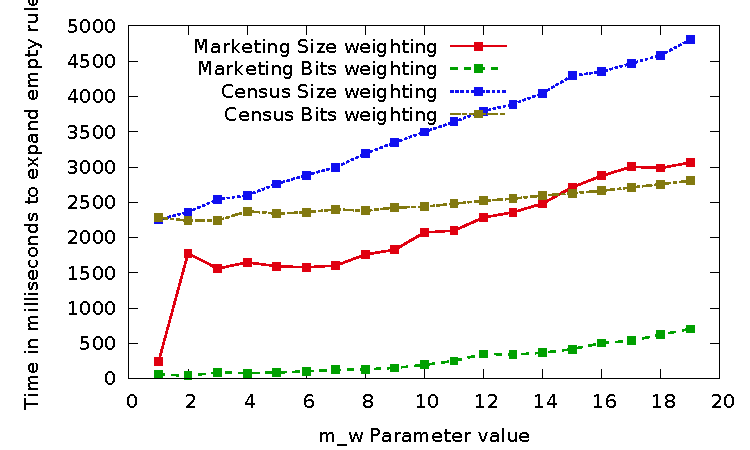
\includegraphics[height=2in]{graphs/mw_speed.pdf}%change height to 2 inch for actual paper, 5 inch for single column
\vspace{-10pt}
  \caption{Running time for different values of parameter $m_w$ \label{fig:mw_speed}}
\vspace{-13pt}
\end{figure}

% TODO: Experiments on m_w. Experiments on Sampling schemes.

\begin{comment}
Notes based on Explanation Tables paper: Prove that our problem is NP-Hard to solve exactly. Something like the Set Cover Problem. 

The way we deal with overlap, is that the key differentiating factor?

We don't have the binary thing. Is it useful? Maybe we can summarize better without it. We are solving a different problem, optimising for coverage rather than explaining the binary attribute. They are optimising for KL divergence of max entropy distribution. They mention many other papers that optimize for cardinality or similar. We do weight times cardinality, which is a compromise between descriptiveness and coverage, and allow user to change the weight function. But should check those papers out anyway. 

\end{comment}

\section{Extensions}
\subsection{Dealing with Numerical Attributes}
Our algorithm assumes that all attributes are categorical in nature. Attributes that have a large domain d to have a smaller tuple count per value, and hence don't appear in rule summaries. Thus our algorithm does not summarise information about numerical attributes. 

However, we can modify the algorithm to deal with numerical attributes. Suppose we have a numerical attribute $A$. A simple approach is to create buckets for values of $A$. We choose a number of buckets $k$, and divide the range of values of $A$ into $k$ intervals, each corresponding to a bucket. We can create buckets having an equal range size, or decide their range such that there is an approximately equal number of tuples in each bucket. Then we can use our algorithm, treating the bucket number as a categorical attribute. This is already done in our MD dataset, where numerical attributes like age are divided into buckets ($18-24$, $25-34$ and so on).

The distribution of values for the $A$ may not be similar in different parts of the table. For instance, we may create buckets have approximately equal numbers of tuples in the table. But then suppose a user tries to expand a rule $r$. The part of the table covered by $r$ might have a very different distribution of age values. For instance, in our MD dataset, if the user looks at people who own a house, their age distribution would be different from that of people who are still renting an apartment. To prevent the buckets from getting a skewed distribution when expanding $r$, we could recompute the bucket ranges every time the user expands a rule, and use the new bucket ranges to determine which rules to display upon expansion. 

\section{Related Work}
%TODO: Repeat what we said in intro about interactive, etc.
There has been work on finding interesting rules in OLAP systems~\cite{Sarawagi:2001:UMA:767141.767148, Sarawagi00user-adaptiveexploration, Sarawagi98discovery-drivenexploration}. The work mainly focuses on finding values that occur more often or less often that expected from a max entropy distribution. The work does not guarantee good coverage of the table, since it rates infrequently occurring sets of values as highly as frequently occurring ones. 

There is work on constructing `explanation tables', which are sets of rules that co-occur with a given binary attribute of the table~\cite{DBLP:journals/pvldb/GebalyAGKS14}. This work again focuses on displaying rules that will cause the max entropy distribution to best approximate the actual distribution of values. 

Our algorithm uses ideas from the a priori algorithm~\cite{apriori}. Several extensions for the algorithm have been proposed, including those for dealing with numerical attributes~\cite{Srikant:1996:MQA:233269.233311}. We can potentially use these ideas to improve handing of numerical attributes in our work. 

% Related Work summary :
% Explanation tables takes lots of papers and talks about them in one go in related work. saying they optimize for different opbjective functions. We can say that as well. We have a unique idea of flexible weighting functions for managing the tradeoff between coverage and specificity. 
% Efficient and Effective... Tableaux

{\small 
\bibliographystyle{plain}
\bibliography{TableSummarization}
}

\end{document}